\documentclass[tikz]{standalone}
\usepackage{amsmath}
\usepackage{xcolor}
\definecolor{bgdark}{HTML}{171D2B}
\definecolor{accent}{HTML}{F7B538}
\color{white}
\pagecolor{bgdark}
\begin{document}
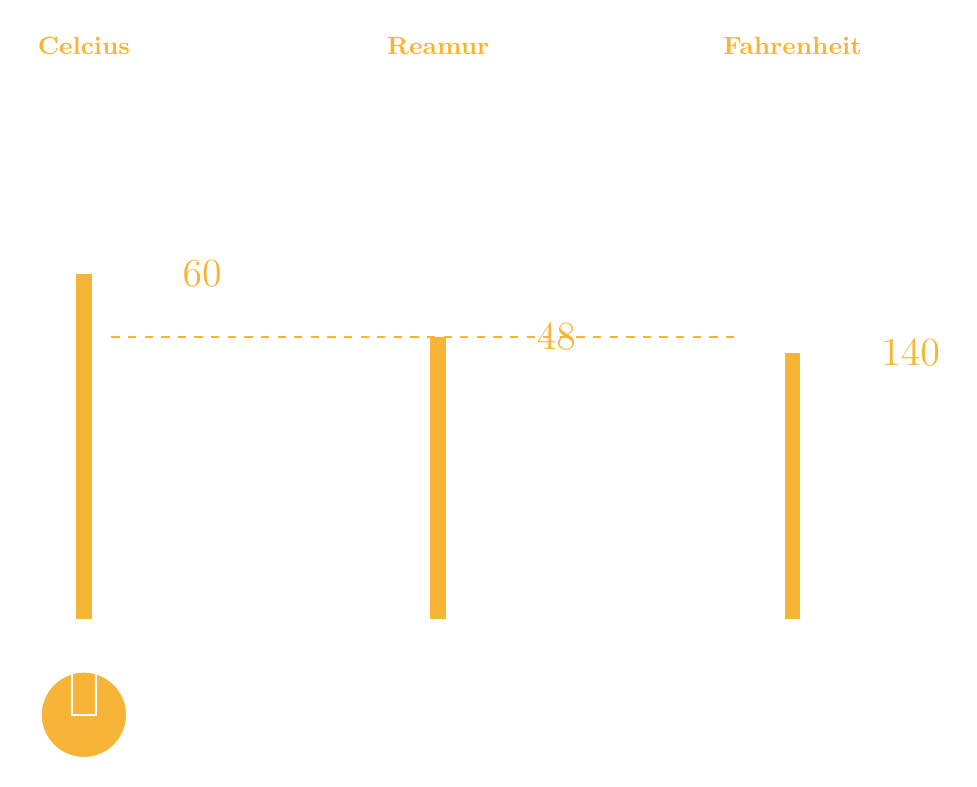
\begin{tikzpicture}[
  scale=1.0,
  tick/.style={white, thin},
  label/.style={white, font=\small},
  scalelabel/.style={accent, font=\small\bfseries},
]
% --- Celcius thermometer (left) ---
\begin{scope}[xshift=0cm]
  \draw[white, thick] (0,0) -- (0,7.6);
  \draw[white, thick] (1.4,0) -- (1.4,7.6);
  \fill[accent] (0.7,-0.2) circle (0.55);
  \draw[white, thick] (0.7,-0.2) circle (0.55);
  \draw[white, thick] (0.55,-0.2) rectangle (0.85,1.0);
  \fill[accent] (0.6,1.0) rectangle (0.8,5.4);
  \draw[white, thick] (0.35,1.0) rectangle (1.05,7.6);
  % ticks every 10 degrees from 0 to 100, scale: 0C at y=1.0, 100C at y=7.0
  \foreach \c in {0,10,...,100} {
    \pgfmathsetmacro{\y}{1.0 + 0.06*\c}
    \draw[tick] (1.05,\y) -- (1.45,\y);
    \node[label, anchor=west, font=\scriptsize] at (1.5,\y) {$\c^\circ$};
  }
  \node[scalelabel] at (0.7,8.3) {Celcius};
  \node[accent, font=\Large] at (2.2,5.4) {60};
\end{scope}

% --- Reamur thermometer (middle) ---
\begin{scope}[xshift=4.5cm]
  \draw[white, thick] (0,0) -- (0,7.6);
  \draw[white, thick] (1.4,0) -- (1.4,7.6);
  \draw[white, thick] (0.35,-0.6) rectangle (1.05,1.0);
  \fill[bgdark] (0.6,1.0) rectangle (0.8,4.6);
  \fill[accent] (0.6,1.0) rectangle (0.8,4.6);
  \draw[white, thick] (0.35,1.0) rectangle (1.05,7.6);
  % Reamur: 0R at y=1.0, 80R at y=7.0 -> 0.075 per degree
  \foreach \r in {0,10,...,80} {
    \pgfmathsetmacro{\y}{1.0 + 0.075*\r}
    \draw[tick] (1.05,\y) -- (1.45,\y);
    \node[label, anchor=west, font=\scriptsize] at (1.5,\y) {$\r^\circ$};
  }
  \node[scalelabel] at (0.7,8.3) {Reamur};
  \node[accent, font=\Large] at (2.2,4.6) {48};
\end{scope}

% --- Fahrenheit thermometer (right) ---
\begin{scope}[xshift=9.0cm]
  \draw[white, thick] (0,0) -- (0,7.6);
  \draw[white, thick] (1.4,0) -- (1.4,7.6);
  \draw[white, thick] (0.35,-0.6) rectangle (1.05,1.0);
  \fill[bgdark] (0.6,1.0) rectangle (0.8,4.4);
  \fill[accent] (0.6,1.0) rectangle (0.8,4.4);
  \draw[white, thick] (0.35,1.0) rectangle (1.05,7.6);
  % Fahrenheit: 32F at y=1.0, 212F at y=7.0 -> (212-32)=180 over 6 -> 0.03333 per F
  \foreach \f in {32,50,...,212} {
    \pgfmathsetmacro{\y}{1.0 + (\f-32)*(6.0/180.0)}
    \draw[tick] (1.05,\y) -- (1.45,\y);
    \node[label, anchor=west, font=\scriptsize] at (1.5,\y) {$\f^\circ$};
  }
  \node[scalelabel] at (0.7,8.3) {Fahrenheit};
  \node[accent, font=\Large] at (2.2,4.4) {140};
\end{scope}

% alignment dashed line at 60C
\draw[dashed, accent, thick] (1.05,4.6) -- (9.0,4.6);
\end{tikzpicture}
\end{document}
